%
%
%
% - - - - - Stand der Technik - - - - - - - - 
%
%
%
\chapter{Stand der Technik}
\label{sec:Stand_der_Technik}
Zur genaueren Einordnung von Smartglasses und deren Klassifikation müssen zunächst einige Grundlegende Begriffe geklärt werden. Smartglasses werden in der Literatur verschiedenen Kategorien zugeordnet. So werden sie als Head-Mounted-Displays (HMD), sowohl dem Wearable Computing als auch des \emph{Ubiquitous Computing} zugeordnet \cite[S.~20]{ThomasDirkMetzgerHelmutNiegemannHrsg2018}. Ubiquitous Computing beschreibt die Allgegenwärtigkeit von Rechnern an jedem Ort, zu jeder Zeit, in jeder Situation und jedem Format. Ziel von Ubiquitous Computing ist es, Computer nicht nur mobiler zu gestalten, sondern zum integralen Bestandteil des Alltags zu machen \cite[S.~24]{Schwenke2016}. Grundvoraussetzung dafür ist nicht nur das \emph{Mobile Computing}, also die überall vorhandene Computerunterstützung, sondern auch das \emph{Pervasive Computing}, also die durchgehende Datenverarbeitung. 

HMD umfassen sowohl Virtual Reality (VR)-Brillen, als auch Augmented Reality (AR)-Brillen.
%
%
%
% - - - - - Einordnung von Smartglasses - - - - - - - - 
%
%
%
\section{Einordnung von Smartglasses}
\label{sec:Einordnung_von_Smartglasses}
Der Begriff \emph{Smartglasses} (oder das deutsche Wort \emph{Datenbrillen}) ist in der Literatur nicht eindeutig definiert und bedarf daher einer Einordnung \cite[S.~26]{Schwenke2016}. Abbildung \ref{fig:Einordnung_Von_Smartglasses} zeigt das Spektrum von Smartglasses in steigender Intensität von Virtual Reality (VR) und Augmented Reality (AR), welches im Folgenden beschrieben wird.
%
\begin{figure}[htbp]
    \centering
    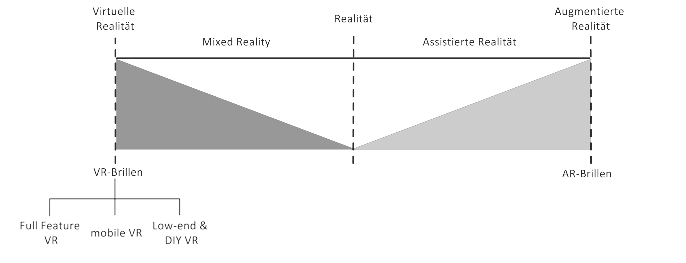
\includegraphics[width=1\textwidth]{data/bilder/VRvsAR.pdf}
    \caption{Einordnung von Smartglasses}
    \label{fig:Einordnung_Von_Smartglasses}
\end{figure}
%
\subsection{Virtual Reality}
%
\emph{Virtual Reality (VR)} ist das völlige Ersetzen der wahrgenommenen Realität durch eine virtuelle Realität. Dabei wird dem Nutzer somit das Gefühl vermittelt, \enquote{Teil einer virtuellen Realität zu sein.} \cite[S.~22]{ThomasDirkMetzgerHelmutNiegemannHrsg2018}. Virtual Reality-Brillen ermöglichen es dem Nutzer im Gegensatz zu Augmented Reality-Brillen komplett in eine virtuelle Realität abzutauchen. 
%
\note{Abtauchen zu salopp.}
%
Realisiert wird dies durch vollständig geschlossene Gehäuse und Linsen, die vor dem Bildschirm befestigt sind. Mittels der Linsen vor dem OLED-Display wird ein scharfes Sehen in einem sehr nahen Bereich ermöglicht. Bei VR-Brillen wird zwischen Full-Feature, Mobile und Low-Budget VR-Brillen unterschieden. Full-Feature Brillen wie die Oculus Rift (Abbildung \ref{fig:OculusRift}) sind mit einer für jedes Auge separaten Full-HD-Auflösung mit hoher Bildwiederholungsrate ausgestattet und bieten dank einer leicht versetzten Anordnung einen dreidimensionalen Effekt. 
%
\begin{figure}[htbp]
    \centering
    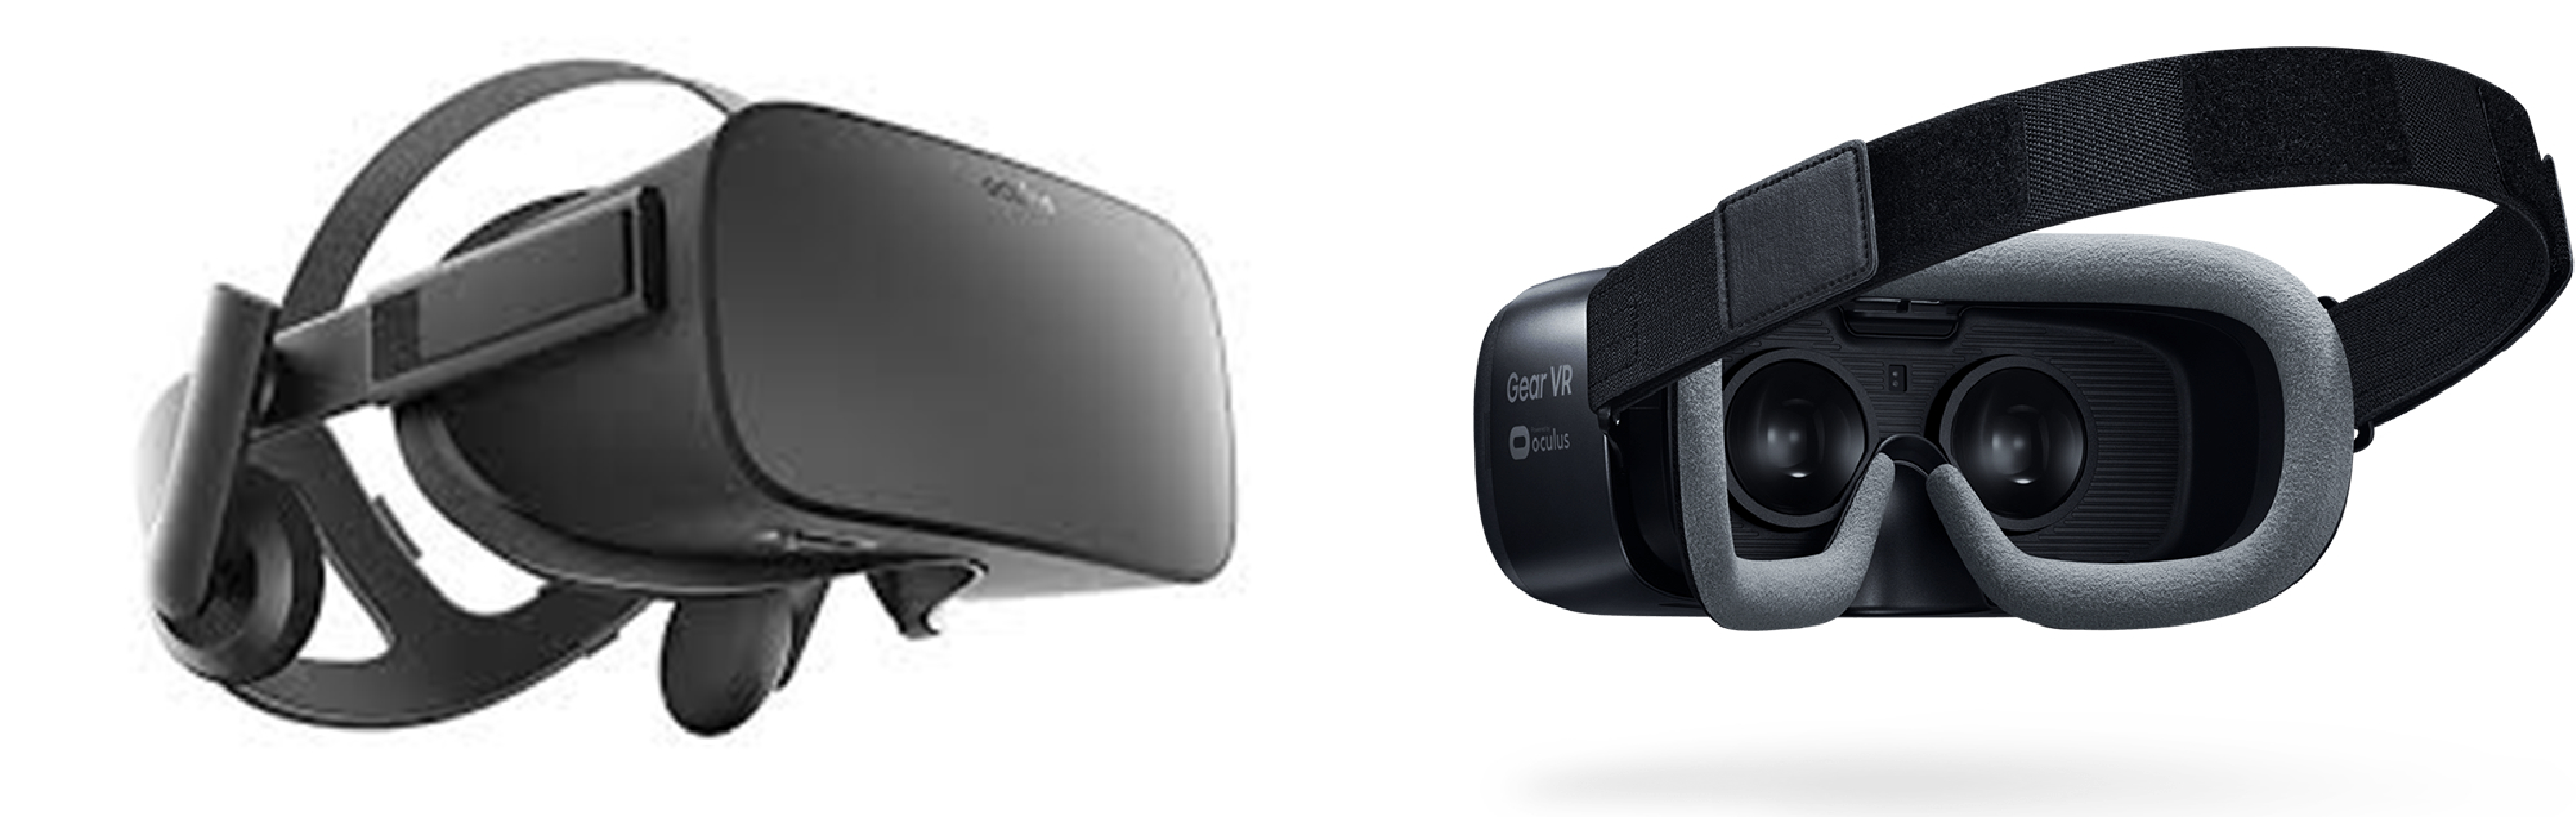
\includegraphics[width=1\textwidth]{data/bilder/Rift_Gear.pdf}
    \caption{Oculus Rift \cite{Oculus2018} (links) und Samsung Gear \cite{Samsung2018} (Rechts)}
    \label{fig:OculusRift}
\end{figure}
%

Der Anwender verliert durch diese Brillen das Gefühl, auf einen Bildschirm zu schauen. Die Außenwelt wird vollkommen ausgeblendet. Bewegungen mit dem Kopf werden automatisch in die virtuelle Welt übernommen. Nutzer bekommen das Gefühl, vollkommen Teil der virtuellen Welt zu sein \cite[S.~22ff]{ThomasDirkMetzgerHelmutNiegemannHrsg2018}. Mobile- und Low-Budget-VR-Brillen wie die Samsung Gear sind Produkte, die mithilfe eines aufgesetzten Smartphones eine Virtuelle Realität erstellen.


%
\subsubsection{Mixed Reality}
%
Unter \emph{Mixed Reality} wird eine Vermischung von realer Umgebung und virtueller Realität verstanden. Dabei wird eine Umgebung erstellt, in der reale und virtuelle Objekte kombiniert werden können. Darunter werden also Brillen verstanden, die komplett geschlossen sind und mittels einer Kamera Inhalte aus der realen Welt in die virtuelle Realität übertragen können.
%
\subsection{Augmented Reality}
%
\emph{Augmented Reality (AR)} ist im Gegensatz zu Virtual Reality das Einblenden von Informationen in das direkte Sichtfeld des Nutzers. Das Blickfeld des Trägers wird also um virtuelle Informationen erweitert \cite[S.~26]{Schwenke2016}. Es wird keine komplett virtuelle Realität erzeugt, sondern die reale Welt um digitale Inhalte ergänzt. Es gibt  unterschiedliche Arten von Brillen, die Augmented Reality-Effekte erzeugen. Differenziert wird zwischen Brillen, die \enquote{echte} Augmented Reality erzeugen und denen, die \emph{unterstützende Realität} erzeugen.
%
\subsection*{AR-Brillen}
%
\enquote{Echte} Augmented Reality wird durch Brillen wie die \emph{Microsoft Hololens} erzeugt. Dabei werden kontextsensitive Informationen direkt im Sichtfeld des Nutzers eingeblendet. Oberflächenerkennung ermöglicht eine Verschmelzung von realer Welt und digitalen Informationen. Die Microsoft Hololens (Abbildung \ref{fig:Microsoft_Hololens}) beispielsweise ist in der Lage, dreidimensionale Hologramme im Sichtfeld des Nutzers anzuzeigen. Dies wird durch zwei transparente Displays ermöglicht. Diese völlige Manipulation der realen Welt wird auch als \emph{Mediated Reality} bezeichnet \cite[S.~46]{Schwenke2016}.
%
\begin{figure}[htbp]
    \centering
    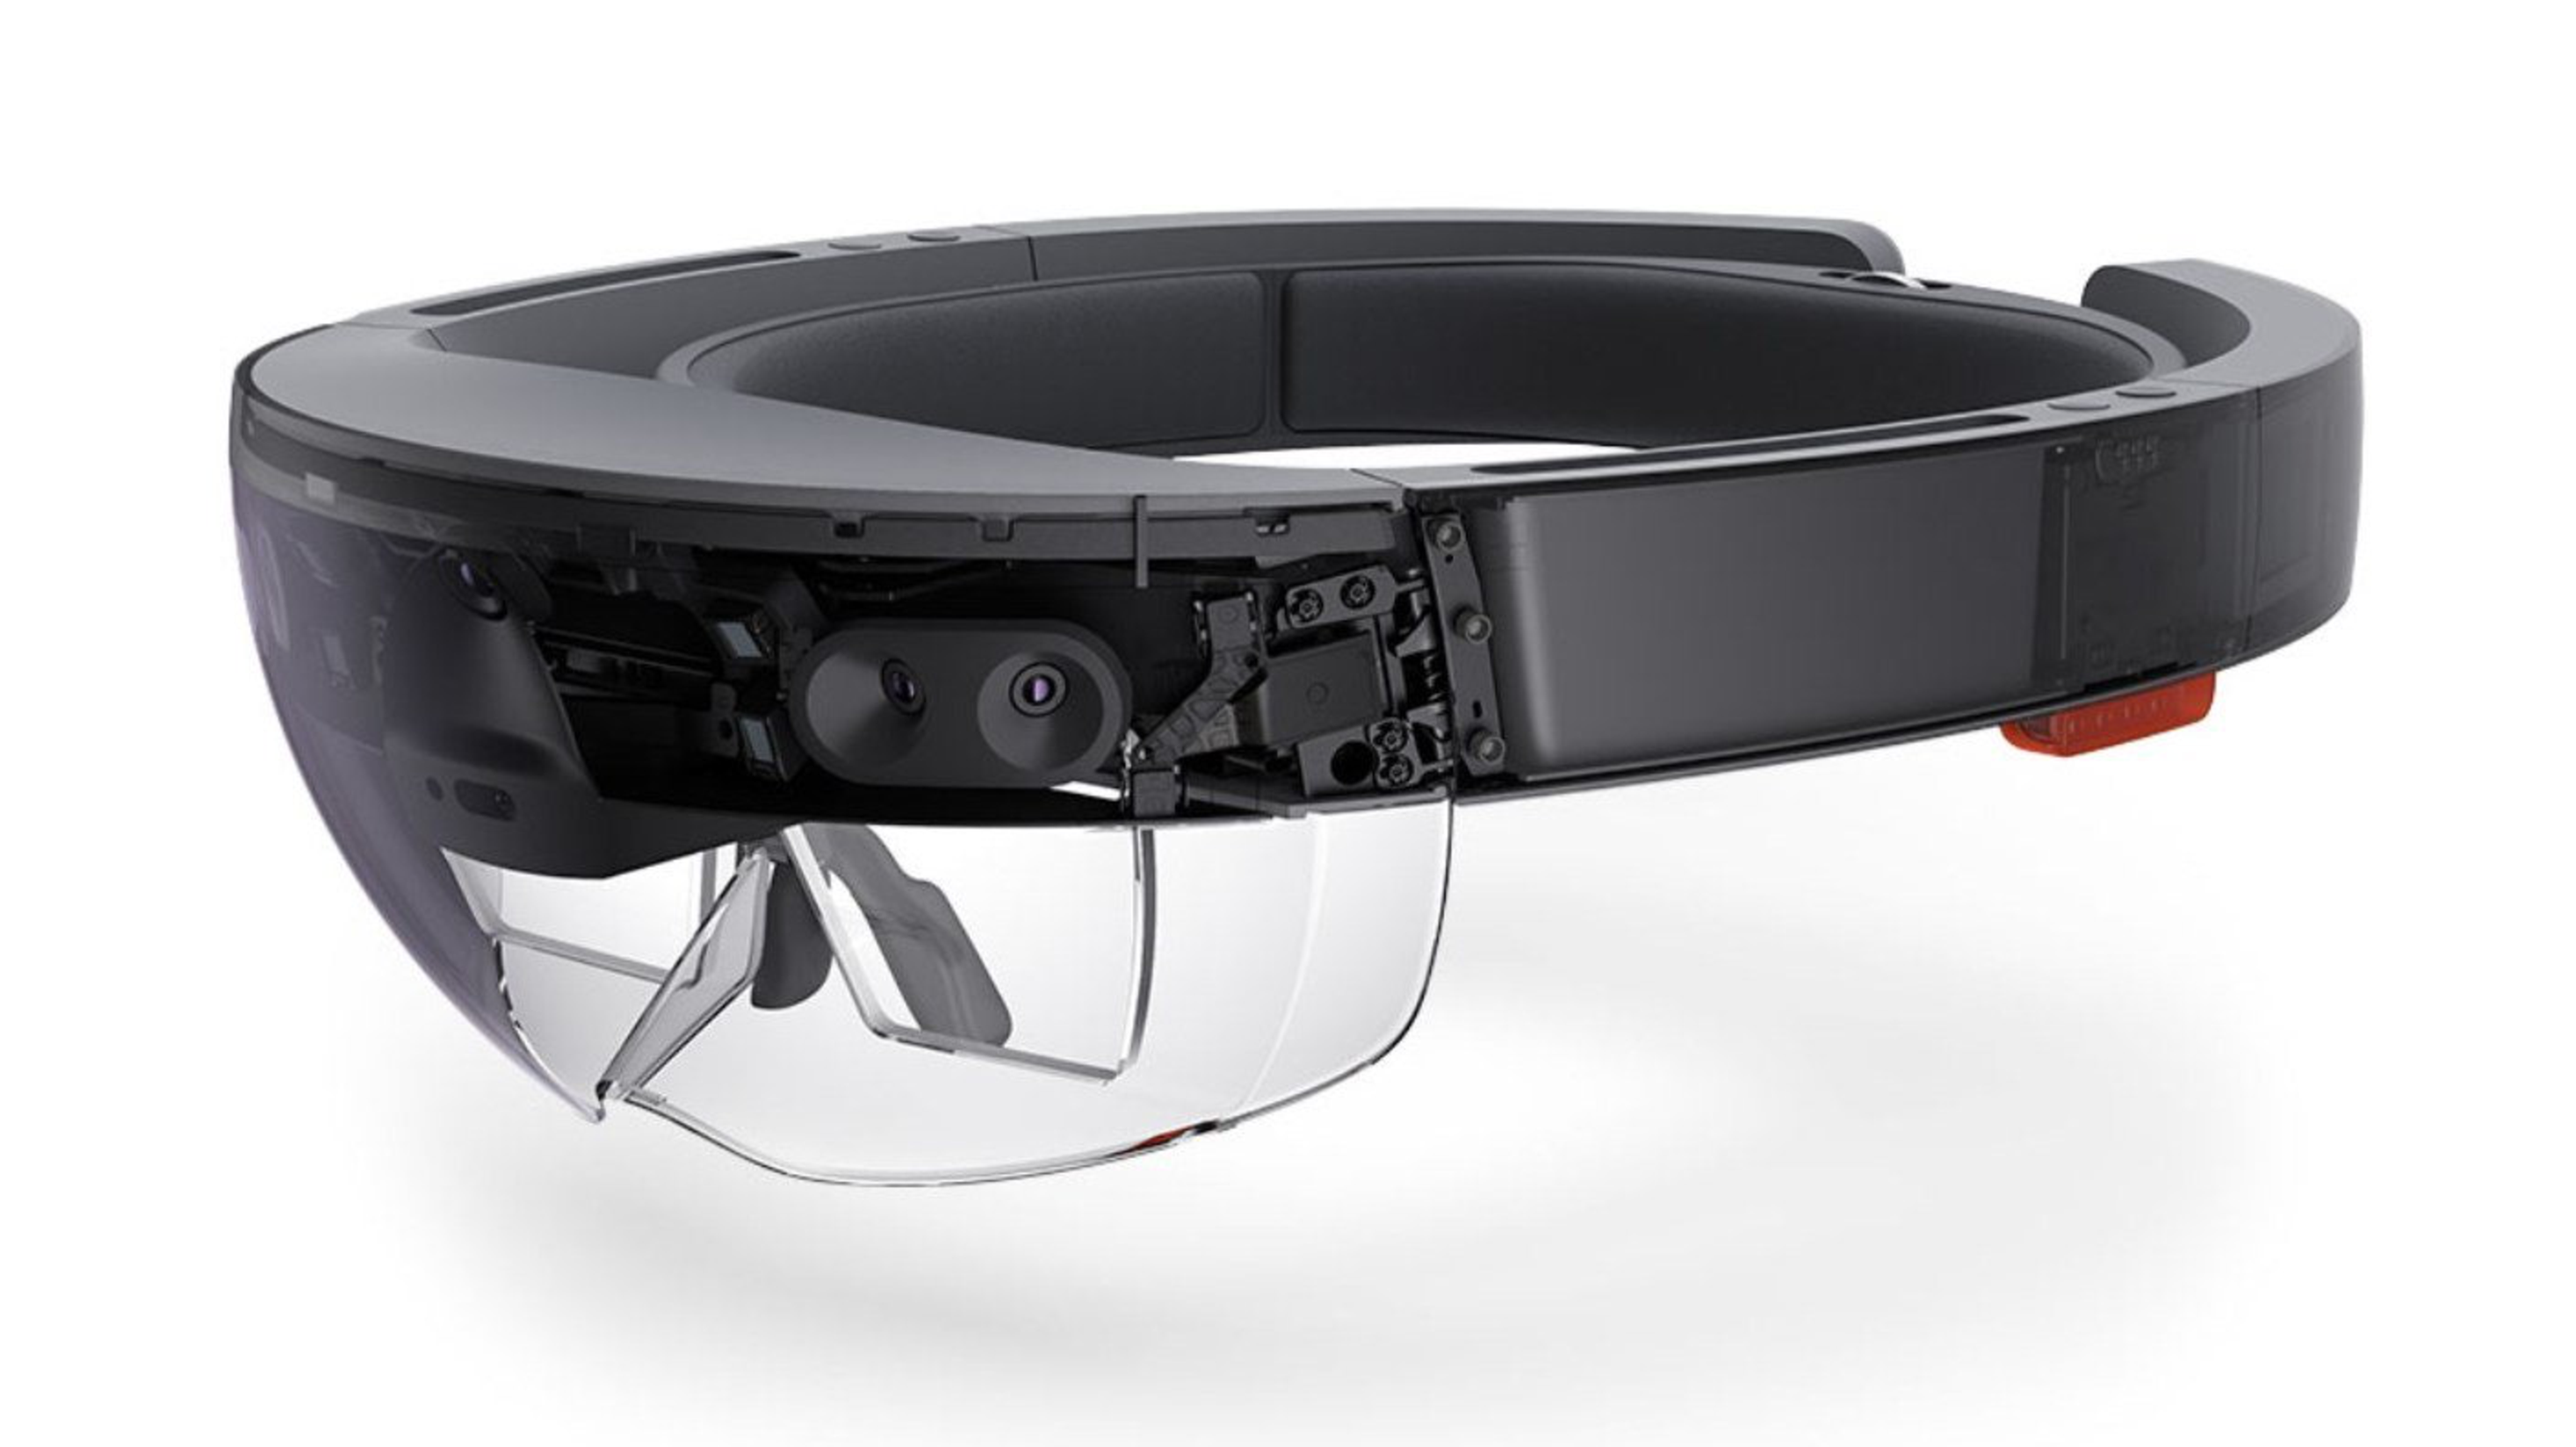
\includegraphics[width=0.5\textwidth]{data/bilder/Microsoft_Hololens.pdf}
    \caption{Microsoft Hololens \cite{O.V.}}
    \label{fig:Microsoft_Hololens}
\end{figure}
%
%

\subsubsection{Assistierte Realität}
\label{sec:AssistierteRealitaet}
%
Von \enquote{echter} AR abzugrenzen ist eine \emph{assistierte Realität}, die beispielsweise durch die \emph{Google Glass}, die \emph{Realwear hmt1} oder die \emph{Epson Moverio BT-200} (vgl. Kapitel \ref{sec:VergleichSmartglasses}) erzeugt wird.

Bei diesen Brillen werden mittels eines sogenannten \emph{Optical Head Mounted See-Through-Displays} \cite[S.~26]{Schwenke2016}, einem Prisma auf einem Auge, virtuelle Inhalte angezeigt, ohne Verlust der Realität mit sich zu ziehen. Im experimentellen Zustand befinden sich Geräte, die Informationen statt auf ein transparentes Display direkt auf die Retina des Auges projizieren \cite[S.~241]{Broll2013}. Ebenfalls zu erwähnen sind am Anfang ihrer Entwicklung befindliche Kontaktlinsen, sogenannte \emph{Smartlenses}, die Informationen mittels LEDs direkt auf die Kontaktlinse bzw. Netzhaut projizieren sollen \cite{Donath2014, Schwan2014}. Im medizinischen Bereich werden bereits heute sub-retinale Implantate getestet, die es ermöglichen, beschädigte Nerven zu ersetzen \cite{Young2013}. Dies ermöglicht ebenfalls die Einblendung von assistierten Realitäten.

Steuern lassen sich AR-Brillen mittels optischer Impulsgeber (\emph{Pick-by-Light}) oder mobiler Hilfsmittel wie Headsets (\emph{Pick-by-Voice}) \cite{INTRALOGISTIK2016}. Es ist also möglich per Gesten- oder Sprachsteuerung zu navigieren. Manche Smartglasses besitzen zudem Touch-Sensoren.

Der Einsatz weiterer Sensoren, wie Trägheitssensoren oder Standortbestimmung sind ebenfalls möglich. Die Kamera einer Smartglass kann zudem über weitere Sensoren, wie Termalsicht, verfügen \cite[S.~27]{Schwenke2016}. Oftmals sind Smartglasses mit WLAN, Mobilfunk oder Nahfeldtechnologien mit dem Internet verbunden oder über Schnittstellen mit einem externen Smartphone verknüpft, welches diese Funktionalitäten bereitstellt \cite[S.~28]{Schwenke2016}.

Für Augmented Reality sind Smartglasses zwar nicht zwingend erforderlich, da diese auch mittels bspw. Smartphones erreicht werden kann. So zeigt Apple mit dem AR-Kit \cite{Apple2018} die technischen Möglichkeiten mittels Augmented Reality in Smartphones. Es ist möglich mit dem Ende 2018 in iOS 12 erscheinenden AR-Kit 2 mit mehreren Nutzern in einer virtuellen über den realen Raum gelegten Realität zu interagieren. Smartglasses bieten jedoch viele Vorteile, da diese die Hände frei halten und die erweiterte Realität direkt vor den Augen des Betrachters und nicht in einem in der Hand befindlichen Smartphone dargestellt wird.

Softwaretechnische Beschränkungen der Smartglass sind grundsätzlich die gleichen, die auch für Android-Smartphones gelten. Auf allen gängigen Smartglasses befindet sich als Betriebssystem Android (vgl. Kapitel \ref{sec:VergleichSmartglasses}). Weitere Beschränkung erfahren Smartglasses lediglich durch die geringe Displaygröße, die eine starke Anpassung einer Anwendung erfordert (siehe Kapitel \ref{sec:Grenzen_des_Einsatzes_von_Smartglasses}).
%
%
%
% - - - - - Smartglasses im beruflichen Umfeld - - - - - - - - 
%
%
%
\section{Smartglasses im beruflichen Umfeld}
\label{sec:Smartglasses_im beruflichen_Umfeld}
% 3 Seiten
Die Logistikbranche ist Deutschlands drittgrößte Branche \cite{Zobel2016}. In der Logistikbranche werden Datenbrillen in Form von Assistierten AR-Brillen eingesetzt \cite{Niemoller2017}.
\\
Smartglasses ermöglichen die Digtialisierung von Arbeitsprozessen und machen es möglich, die Integration von Mitarbeitern in Unternehmensprozesse zu verbessern \cite{Zobel2016}. Sie liefern Kontextabhängige Informationen, beispielsweise via Barcodes bzw. QR-Codes. Angestellte der Logistikbranche der Transportlogistik werden so in Echtzeit mit Informationen, wie beispielsweise Lieferaufträgen versorgt. In einer Use-Case-Studie von Niemöller \cite{Niemoller2017} wurden insgesamt 36 Einsatzmöglichkeiten für Smartglasses im Logistikdienstleistungssektor ermittelt. Die relevantesten Use-Cases werden im Folgenden dargestellt:
\\
Zum einen wurde das Themenfeld Kommunikation herausgearbeitet. Mittels Smartglasses ist das Anzeigen von Handlungsanweisungen sowie die Darstellung von Videoinformationen mittels Streaming oder Offlinevideos möglich. Eine vereinfachte Kommunikation durch die Übersetzung von Texten ist ebenso möglich. Im Themenfeld Qualitätssicherung ist eine automatisierte Kontrolle mittels einer kamerabasierter Fehlererkennung sowie entsprechender Rückmeldung an den Nutzer möglich. Das Haupteinsatzfeld ist jedoch die Identifizierung anhand gespeicherter Merkmale wie Farbe, Größe und Geometrie oder auch durch die Identifizierung mittels Bar- und QR-Codes \cite{Niemoller2017}. Identifizierung von Objekten ermöglicht die Anzeige von Zusatzinformationen. Im Themenfeld Sicherheit ist die Kontextabhängige Darstellung von Sicherheits- und Warnhinweisen möglich. 

Auf dem Fachkongress \emph{Smart Glasses Experience Days} \cite{Manokaran-Pathamathan2017} wurden weitere Einsatzfelder aufgezeigt. So können über die Datenbrille Montage- oder Reparaturanleitungen angezeigt werden. Zwecks Dokumentation werden Arbeitsschritte und Informationen des vorhergehenden Angestellten angezeigt. Per Remoteunterstützung können Angestellte Hilfe bei komplizierten Arbeitsschritten erhalten. Es können für Lagermitarbeiter Anweisungen angezeigt werden, wie und in welcher Reihenfolge Anweisungen befolgt werden sollen.

Neben der Logistikbranche werden Smartglasses auch in anderen Branchen eingesetzt. In dem Studienbericht \emph{Smart Glasses in der Produktion} des Fraunhofer-Instituts für Produktionstechnologie IPT von 2016 \cite{Plutz} wurde der Einsatz von Smartglasses im beruflichen Umfeld der industriellen Produktion analysiert. So setzen 3,4\% der 237 befragten Unternehmen  Smartglasses bereits ein. 15,1\% wollen diese in nächster Zeit einsetzen. Die häufigsten Anwendungsgebiete waren Mitarbeiterschulungen (27,3\%), Fernwartung/Videotelefonie (27,1\%), Echtzeitanzeige von Informationen (22,8\%) und industrielle Bildverarbeitung (17,5\%). Laut dem Bericht ist es möglich, nicht nur 
prozessrelevante Informationen zur Verfügung zu stellen, sondern Angestellte auch dazu zu befähigen, Informationen prozessintegriert zu erzeugen. Es sei zudem möglich, hoch aufgelöste Zeiterfassung manueller Tätigkeiten zu realisieren und Prüfdaten nicht wie bislang handschriftlich zu erfassen, sondern dabei die Hände frei zu haben.

Laut einer Pressemitteilung des Logistikunternehmens DHL vom 2. August 2017 führt der Einsatz von Smartglasses zu einer 15-prozentigen Produktivitätssteigerung bei geringerer Fehlerquote \cite{DeutschePostDHLGroup2017}. Mittels Sprachsteuerung lassen sich einzelne Kommissionieraufträge aufrufen und die nötigen Informationen auf dem Display anzeigen. So lassen sich Lagerort, Lagerplatz und die zu packende Anzahl der Ware anzeigen statt wie bisher auf papierbasierte Auftragsanweisungen zurückgreifen. 

Das Unternehmen Bosch setzt in ihrer Logistiksparte ebenfalls Smartglasses ein. Für Bosch ist vor allem die Tatsache von Vorteil, dass die Angestellten beim Scannen von Barcodes und QR-Codes freihändig agieren können \cite{Spinger2014}. 
%
%
%
% - - - - - Vergleich verschiedener Smartglasses - - - - - - - - 
%
%
%
\section{Vergleich verschiedener Smartglasses}
\label{sec:VergleichSmartglasses}
% 2 Seiten
Da in dieser Arbeit Augmented Reality-Brillen und insbesondere Smartglasses mit assistierter Realität (\ref{sec:AssistierteRealitaet}) behandelt werden, werden im Folgenden einige Brillen dieses Bereiches vorgestellt.
%
%
%
% - - - - - - - - Google Glass - - - - - - - - - - - -
%
%
%
\subsection{Google Glass}
\label{sec:Google_Glass}
Der 2012 eingeführte Prototyp einer ersten Version von Google Glass (\enquote{Explorer Edition}) hat ein über dem rechten Auge plaziertes durchsichtiges quaderförmiges Display. Neben dem Display befindet sich eine hochauflösende Kamera sowie ein Mikrofon. Im Bügel der Brille ist die Recheneinheit angeordnet. Die Batterieleistung der Brille betrug beim ersten Prototypen nur wenige Stunden, ist in neueren Versionen jedoch deutlich erhöht worden. Die Brille ist mit WLAN ausgestattet und ermöglicht mittels einer Verknüpfung mit einem Android-Smartphone die Verbindung ins Mobilfunknetz sowie die Standortbestimmung mittels GPS.
%
\begin{figure}[htbp]
    \centering
    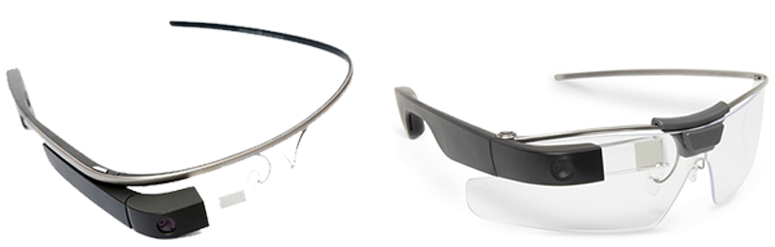
\includegraphics[width=0.8\textwidth]{data/bilder/Glass_1_und_2.png}
    \caption{Google Glass 1 (\enquote{Explorer Edition}) \cite{Reckmann2014a} (links) und Glass Enterprise Edition \cite{Huvelin2017} (rechts)}
    \label{fig:GlassModel}
\end{figure}
%

Die Brille lässt sich über verschiedene Sensoren steuern. So besitzt sie ein Touchpad im Bügel der Brille. Sprachbefehle ermöglichen ebenfalls die Steuerung der Brille. Augenbewegungen des Nutzers werden durch einen Infrarotsensor erfasst. Die Kameraaktivität wird nicht angezeigt \cite[S.~30]{Schwenke2016}. Die Glass ist mit einem Android-Betriebssystem ausgestattet. Es gibt eine ausführliche Dokumentation mit speziellen APIs zur Entwicklung spezieller Glass-Anwendungen.

Mittlerweile hat Google eine speziell für den professionellen Einsatz optimierte Brille veröffentlicht, die \enquote{Glass Enterprise Edition} \cite{Inc.2018}. Diese Brille ist nur für den professionellen Einsatz zugelassen und wird nicht an Privatpersonen verkauft.
%
%
%
% - - - - - Epson Moverio BT-200 - - - - - - - - 
%
%
%
\subsection{Epson Moverio BT-200}
\label{sec:Epson_Moverio_BT-200}
Die Smartglass \emph{Moverio BT-200} von Epson hat im Gegensatz zur Google Glass zwei Bildschirme (je ein Bildschirm vor jedem Auge). 
%
\begin{figure}[htbp]
    \centering
    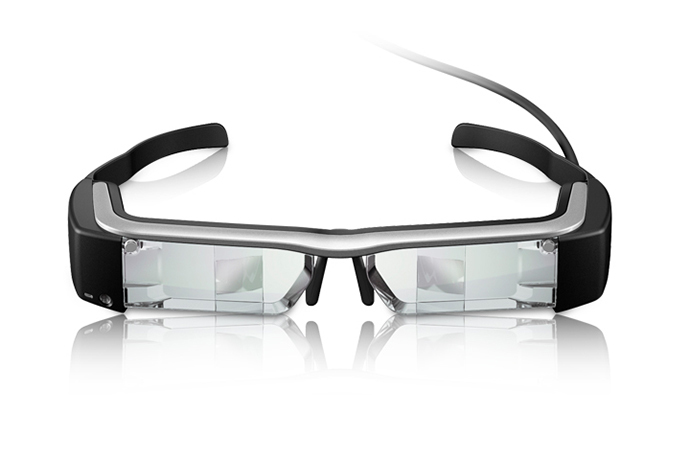
\includegraphics[width=0.4\textwidth]{data/bilder/Moverio_BT-200.png}
    \caption{Epson Moverio BT-200 \cite{Epson}}
    \label{fig:BT-200}
\end{figure}
%
Der Prozessor sowie die Batterie sind extern mittels eines Kabels mit der Brille verbunden. Die Brille verfügt über ein Touchpad, welches ähnlich dem der Google Glass am Bügel der Brille befestigt ist. Die Kamera der Brille ist deutlich geringer aufgelöst (640x480 Pixel), zeigt die Benutzung jedoch im Gegensatz zur Google Glass über eine kleine Leuchtdiode an. Wie auch bei der Google Glass ist das Betriebssystem der Moverio BT-200 Android \cite[S.~32]{Schwenke2016}. Diese Smartglass ist momentan nur in einer Developer-Edition erhältlich \cite{Epson}.
%
%
%
% - - - - - Vuzix M300 - - - - - - - - 
%
%
%
\subsection{Vuzix M300}
\label{sec:Vuzix_M300}
Die \emph{Vuzix M300} ist speziell für den professionellen Einsatz konzipiert. Sie verfügt über ein nicht-Transparentes Display am rechten Auge, hat eine HD-Kamera und großen internen Speicher. Sie ist spritzwassergeschützt und nach Herstellerangaben robust gestaltet. Die Brille verfügt über ein Touch Pad sowie zwei Mikrofone zur Sprachsteuerung. 
%
\begin{figure}[htbp]
    \centering
    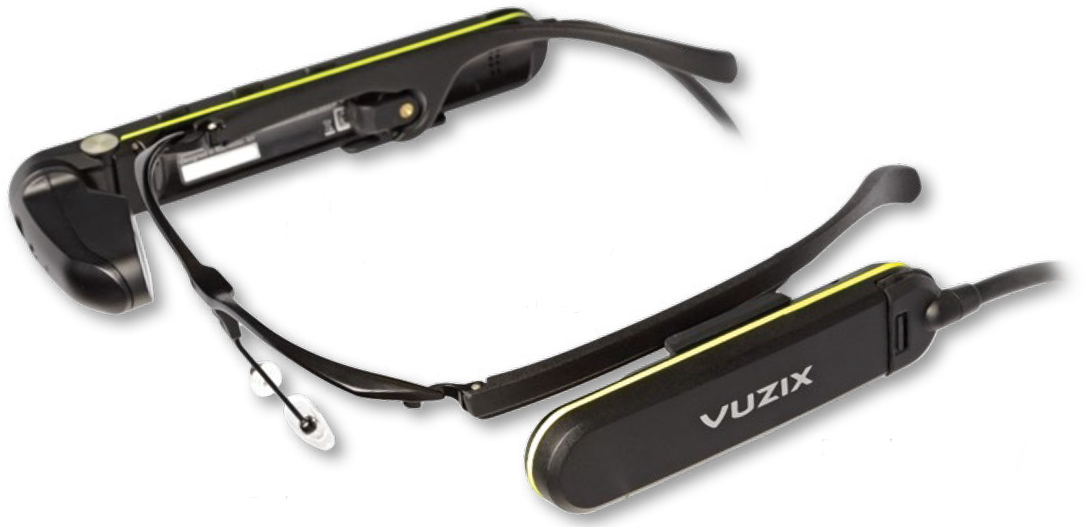
\includegraphics[width=0.4\textwidth]{data/bilder/m300-top.png}
    \caption{Vuzix M300 \cite{Vuzix2018}}
    \label{fig:Vuzix_M300}
\end{figure}
%

Die Vuzix M300 verfügt über schnell austauschbare Akkus, die je nach Anwendungszweck dynamisch angesteckt werden können. So gibt es je nach Anforderung verschieden schwere Akkus. Dies ermöglicht den Einsatz der Brille über einen beliebig langen Zeitraum.

Das Betriebssystem der Brille ist ebenfalls Android. Es lassen sich grundsätzlich alle für Android 6 konzipierten Apps auf der Brille bedienen, jedoch auch speziell für die Brille entwickelte Apps. Die Brille kann mit iOS- und Android-Smartphones gekoppelt werden, um Zugriff auf GPS und Mobilfunk zu erhalten. Zur Entwicklung für die App steht Entwicklern eine weitreichende Dokumentation sowie spezielle APIs zur Verfügung. \cite{Vuzix2018}
%
%
%
% - - - - - Realwear hmt-1 - - - - - - - - 
%
%
%
\subsection{Realwear hmt-1}
\label{sec:Realwear_hmt-1}
%
\begin{figure}[htbp]
    \centering
    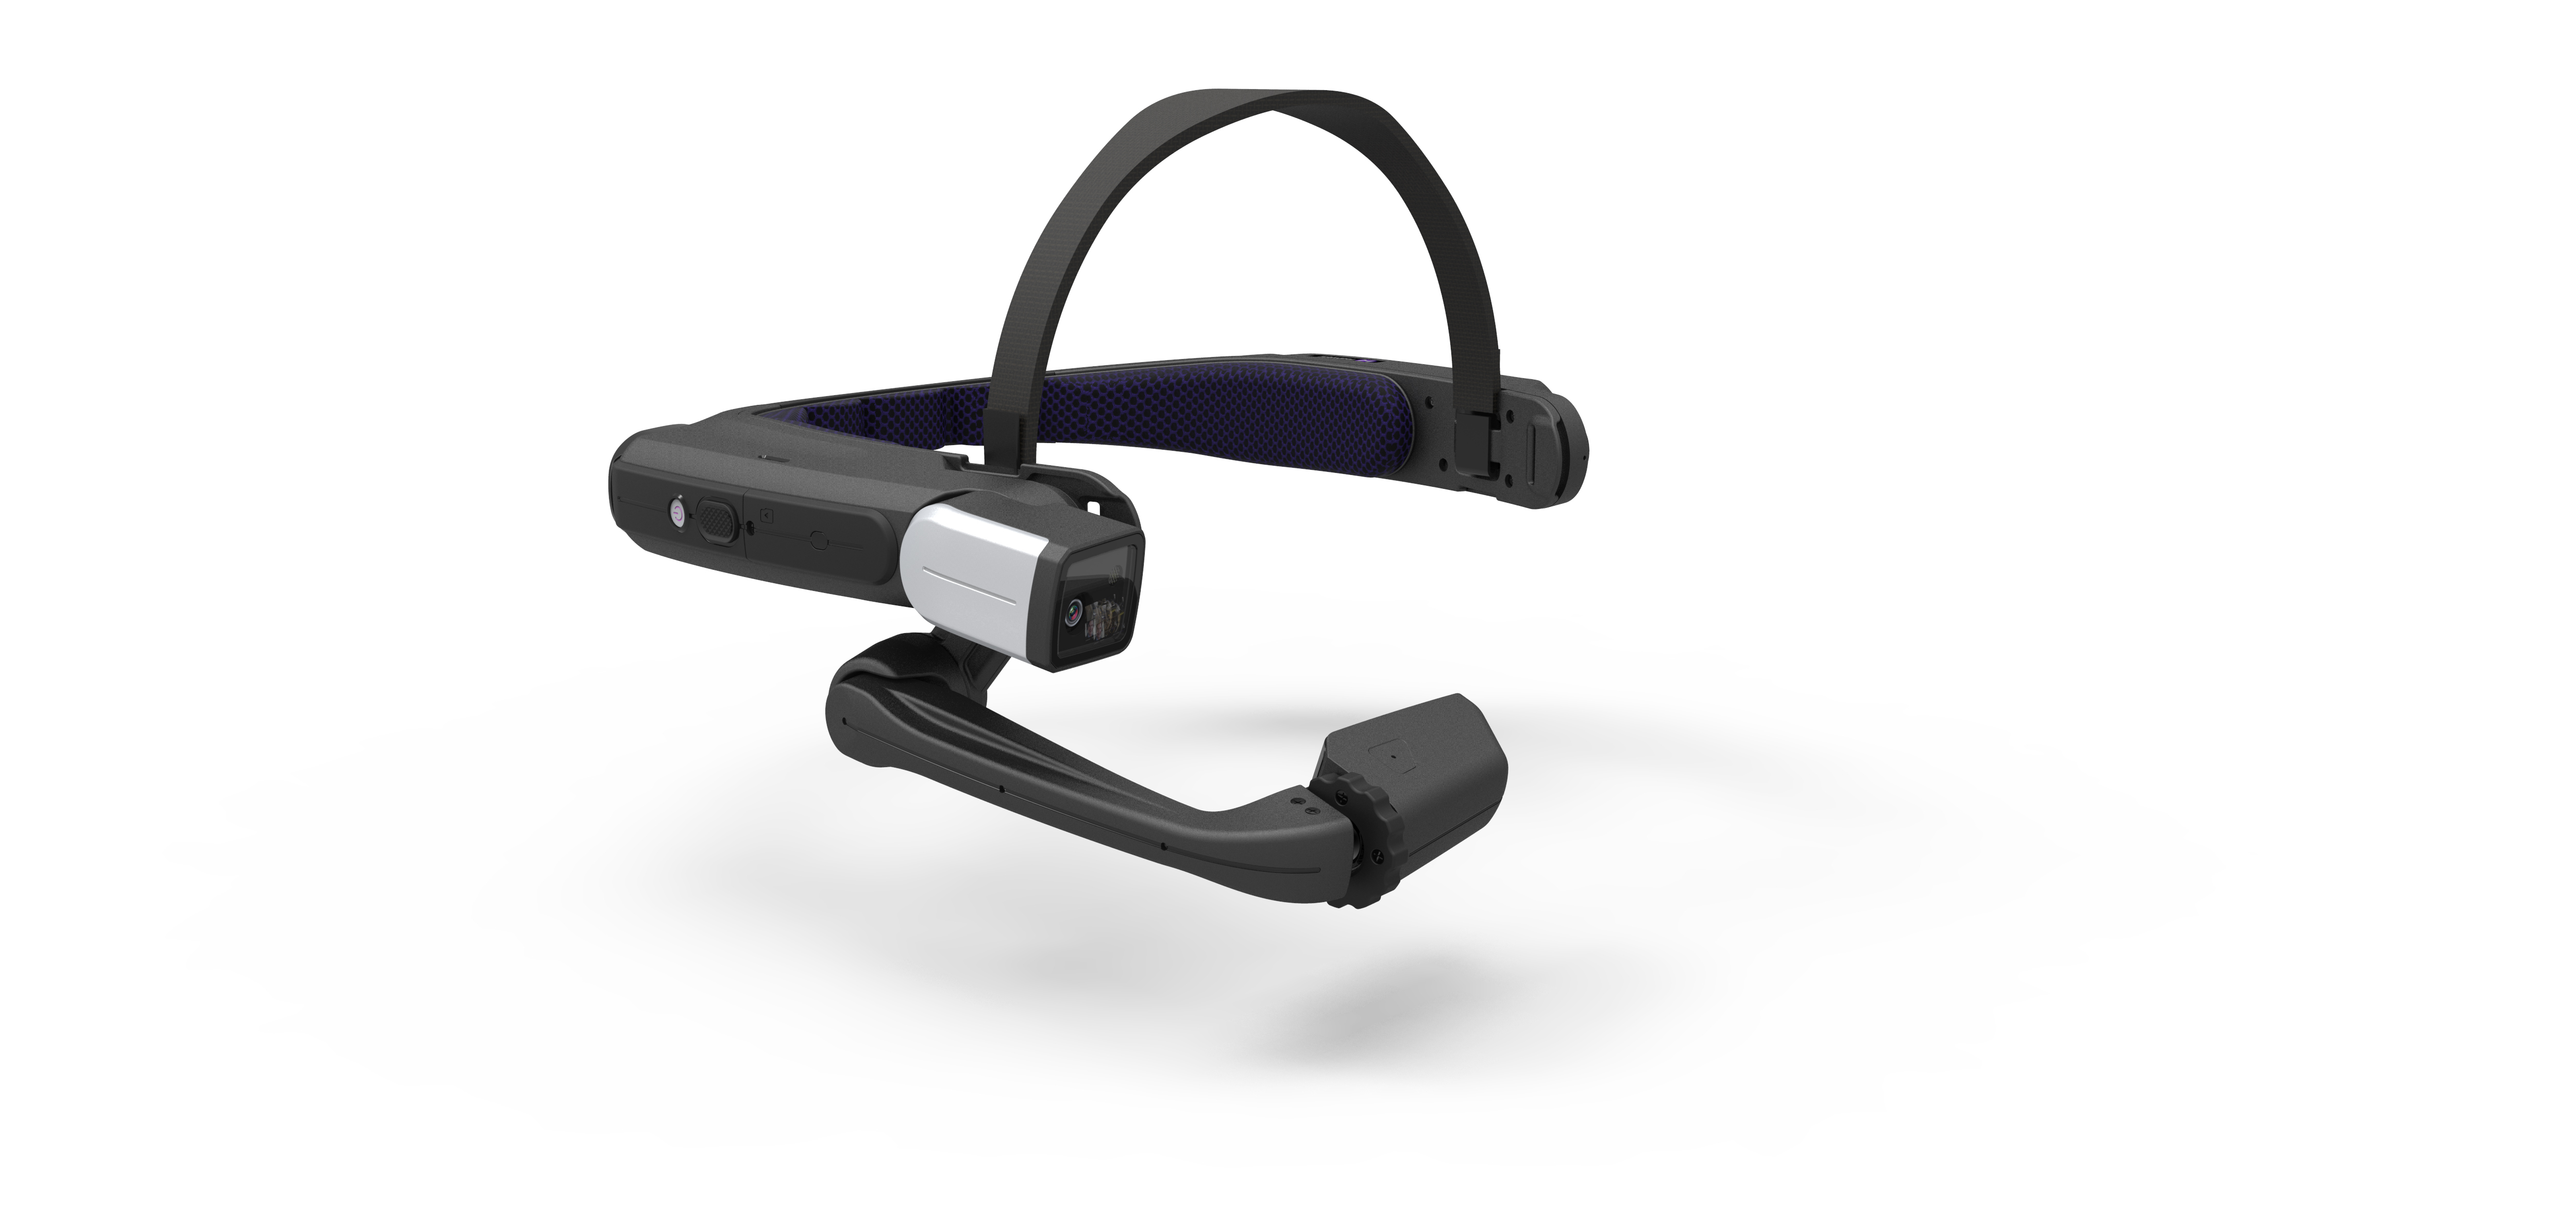
\includegraphics[width=0.9\textwidth]{data/bilder/HMT_1.jpg}
    \caption{Realwear hmt-1 \cite{Wire2017}}
    \label{fig:hmt1}
\end{figure}
%

Die \emph{Realwear hmt-1} ist ebenfalls für den professionellen Einsatz optimiert. Ähnlich der Google Glass ist ein Display am rechten Auge befestigt. 

Im Gegensatz zur Glass ist dieses Display jedoch nicht transparent, es ist jedoch für den Außeneinsatz konzipiert und ist auch bei starkem Sonnenlicht nutzbar. Die Brille ist vollständig abwischbar.

Prozessor und Batterie sind im Bügel der Brille befestigt. Die Brille  besitzt eine Sprachsteuerung mit integrierter Noice-Cancellation mittels vier eingebauter Mikrofone. Die Batterie der Brille hält einen gesamten Arbeitstag. Im Gegensatz zur Glass und BT-200 ist die hmt-1 sturzbeständig auf 2~m. Wie auch Glass und BT-200 ist das Betriebssystem der hmt-1 Android. Es gibt eine gut dokumentierte Entwicklerdokumentation und spezielle APIs zur Entwicklung von speziell für die Brille konzipierten Android-Anwendungen \cite{Realwear2018}.
%
% Hier würde ich noch irgendwie 2 3 Abschließende Sätze bringen, damit eine Überleitung entsteht. Da die Glasses im Bereich der ZSVA eingesetzt werden soll und somit diverse Anforderungen XYZ erfüllen müssen, wird zunächst erläutert wie was die ZSVA ist und wie sie arbeitet... (also irgendwie so). Finde es wichtig in nächste Kapitel überzuleiten. Sonst ist hier ein Cut und es geht mit etwas ganz anderem weiter.